%========================= LIMIT STATE DESIGN ========================%
\chapter{Limit State Design-Introduction}
\section{Reinforced Concrete Codes}

Indian Standard Code of Practice for Plain and Reinforced Concrete was 
first published in 1953 and its second revision \citetitle{is4562000}
is referred here in after as the old code, While its third revision
was made in 1978 and is fourth and the latest revision
\citetitle{is4562000} is called here in after as the new code or
simply the Code. \citetitle{is4561964} mainly deals with the
working stress method of design of reinforced concrete and gives the 
ultimate load method of design in its Appendix B. But the position of 
these two methods of design is reversed in the new code. The working 
stress method is relegated to Appendix B of the Code, while the limit
state method, which is a rationalisation of the ultimate load method, 
forms the main body of the Code. In general, working stress method leads
to a more conservative design than that by the limit state method. This 
manual concerns itself with the limit state method as given in Section
5 of the Code.

\section{Requirements of Design}

All structures must be designed to be safe, serviceable and economical.
Safety means that structures must not fail under loads unless exceeded 
by a given margin called overload safety factors. Serviceability means 
that structures must perform well throughout their service life in both
appearance and comfort to their users. This requirement includes cracking
and deflection under working loads. Economy means that structures must be 
designed in such a way as to minimise the quantities of materials used in
them. Although safety and serviceability are the basic requirements, the 
test of an acceptable structural design is economy.

In design of reinforced concrete structures, all critical sections are
checked for the effect of forces acting on them. So, the economy of
design achieved here refers to the critical sections. his approach in
itself may make a marginal difference, say, within 5\% of cost of
structure, which in itself, is about 40\% to 50\% of the total cost of
building. More substantial economies in cost of structures are achieved 
by the correct choice of structural systems like load-bearing walls,
frames, shear walls and their several combinations. Also, sizing of
columns and beams and spacing of frames in framed buildings will affect
the economy. These decisions will be crucial for economy of structures,
but these are beyond the scope of this manual.

\section{Limit State Method}

Limit state method includes consideration of structures at both the
working and the ultimate load levels with a view to satisfy the
requirements of safety and serviceability. It offers an integrated
approach to design of structures. A reinforced concrete section needs 
to %\footnote{*The number on top refers to Reference given in Appendix B.}
be checked for forces acting on it, together with relevant serviceability
requirements. Each force or a serviceability requirement is called a 
limit state. The aim of design is to ensure that a reinforced concrete
section does not reach any of the limit states to which it may be subjected.
The usual approach is to design a section for a limit state which is
likely to govern it and then check it for the remaining limit states.
The Code gives principles for design of reinforced concrete sections
under the following limit states : 

\begin{enumerate}[(i)]
\item Flexure
\item Compression
\item Axial load and uniaxial bending
\item Axial load and biaxial bending
\item Shear
\item Torsion
\item Deflection
\item Cracking
\end{enumerate}

Limit states (i) to (vi) refer to ultimate limit states or limit states
of collapse, while the last two limit states refer to serviceability 
requirements. Limit state of tension, as may occur in design of concrete 
hangers or suspenders, is not given by the Code. The other relevant limit
states for concrete structures can be impact, vibration, fatigue,
durability, fire-resistance, lightning etc. These limit states are 
satisfied by good quality concrete, adequate size of members, adequate
cover to reinforcement, provision of minimum steel area and other special
details. Limit state of cracking is satisfied by adhering to the
requirements of minimum steel area and spacing of bars in members. Thus,
analysis of reinforced concrete sections under the various ultimate limit
states (i) to (vi) is required. Further, limit state of deflection, which
is crucial for bending members—slabs and beams—needs consideration in 
detail.

\section{Safety Factors}

The system of partial safety factors is followed in the
\citetitle{is4562000} as against the system of unified safety factors
followed in the old code. The values of partial safety factors Yf for
loads are given in \tablem 18 of the Code, which are valid for various
load-combinations mentioned therein. \tablem 18 of the \citetitle{is4562000}
gives ultimate loads for the two common load-combinations as
follows:

\begin{equation}
UL = 1.5 (DL + LL)\\
UL = 1.2 (DL + LL + WL or EL)
\end{equation}

The values of partial safety factors for loads are to be supplemented
with partial safety factors

\begin{align}
\gamma_m (concrete) = 1.50\\
\gamma_m (steel) = 1.15 
\end{align}
The \citetitle{is4561964} gave values of 1.85 and 1.4 as factors of
safety for total loads for the two load-combinations considered in
\eqn 1.1 and \eqn 1.2 respectively and practical examples of design of
slabs and singly reinforced beams show, that these compare well with the
systems of partial safety factors incorporated in the
\citetitle{is4562000}.

\section{Stress-Strain Diagrams for Materials}

\fig 21 of the Code gives the stress-strain diagram for concrete which
is rectangular-parabolic in shape. The design strength at the extreme
fibre in compression is given by,

\begin{equation}
f_c = 0.67\frac{f_{ck}}{\gamma_m} = 0.67\frac{f_{ck}}{1.5}=0.45 f_{ck}
\end{equation}
Where, $f_{ck}$ is the characteristic cube strength of concrete in
compression at 28days. The factor 0.67 in \eqn 1.5 accounts for
variation in strength of concrete in actual structure as against
that in the cube test of concrete. \eqn for concrete stress diagram
of \fig 21 of the Code is given with reference to \eqn 1.1. For the
range x = O to g (A to B),

\begin{figure}
\begin{subfigure}{0.5\textwidth}
\centering
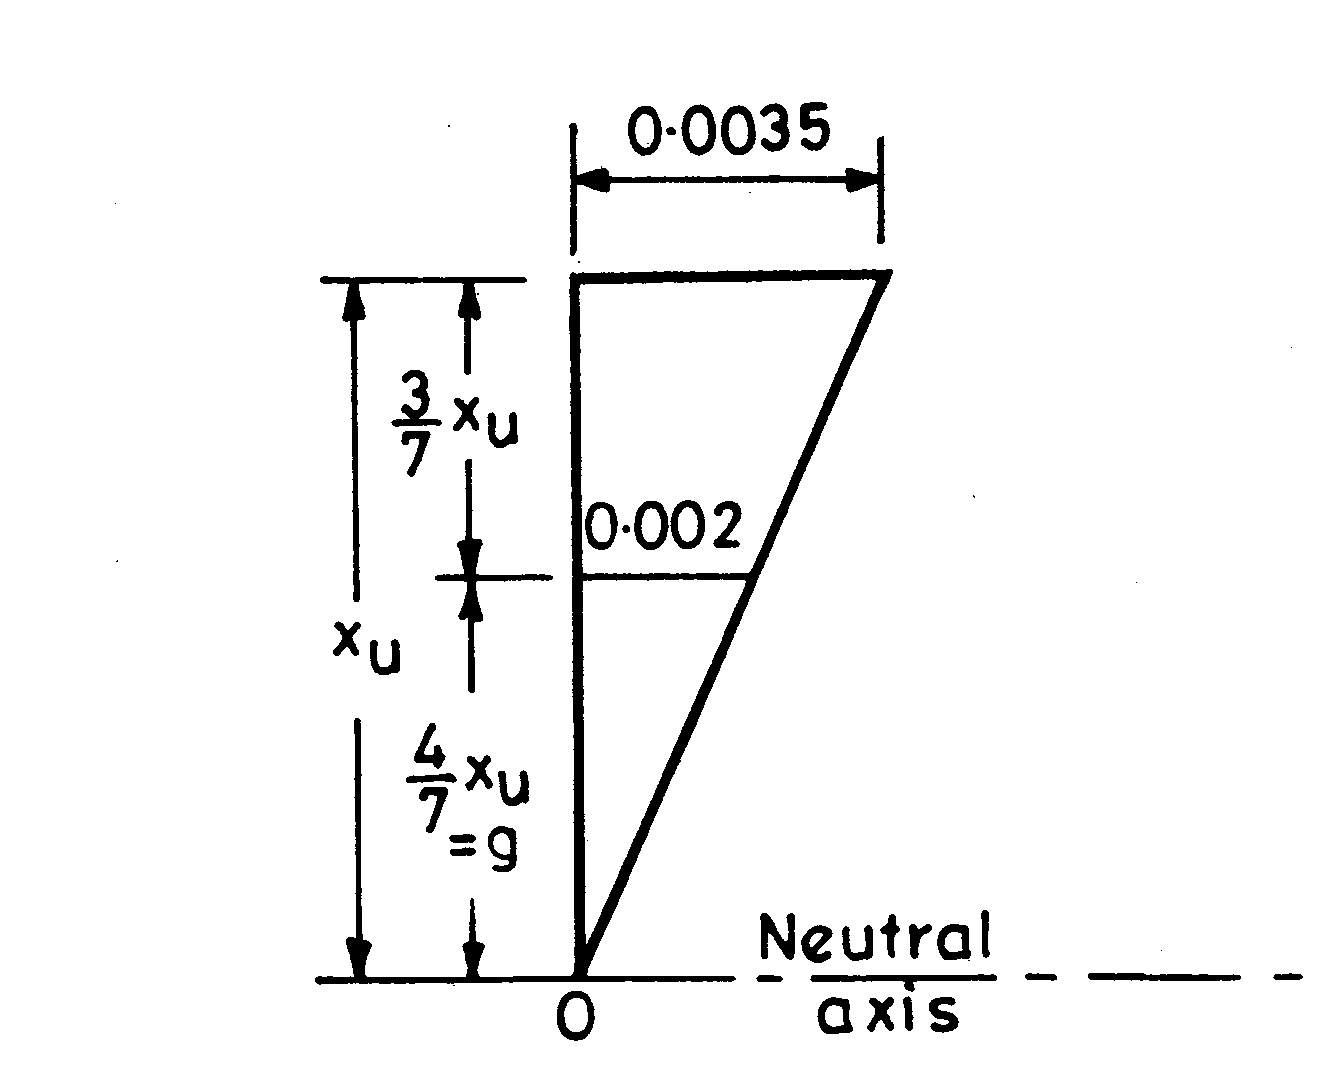
\includegraphics[width=\textwidth]{images/linear.png}
\caption{Linear concrete strain diagram}
\label{fig:linear}
\end{subfigure}
%
\begin{subfigure}{0.5\textwidth}
\centering
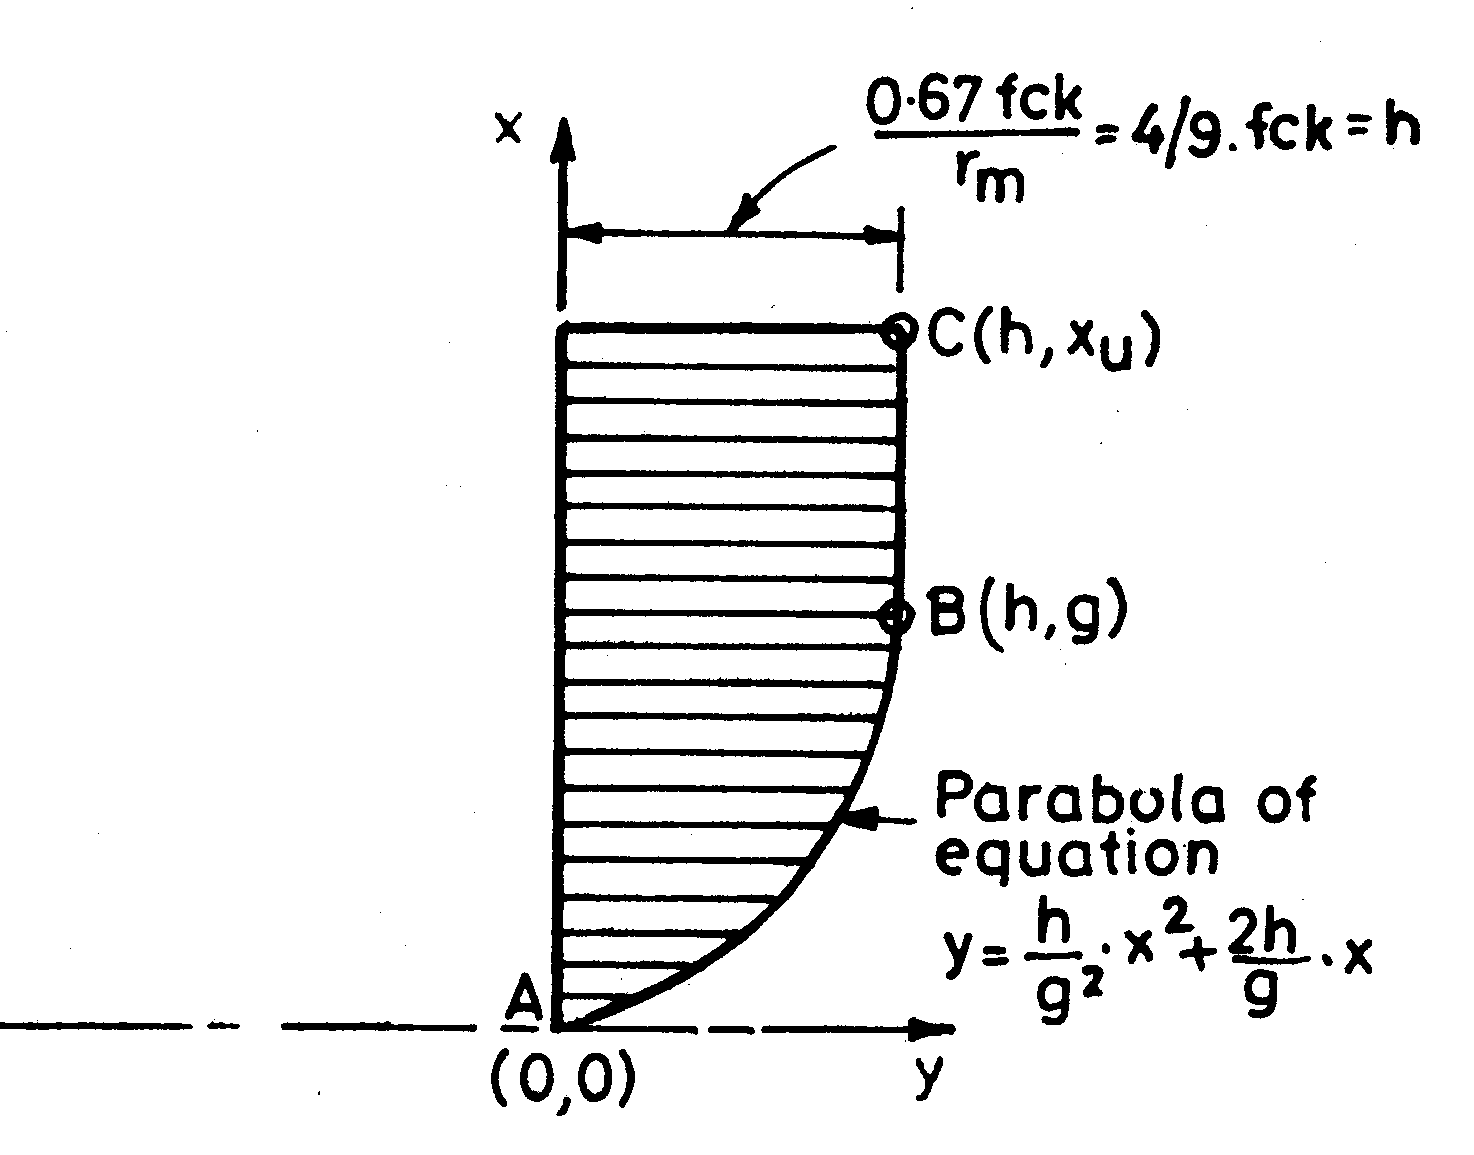
\includegraphics[width=\textwidth]{images/parabolic.png}
\caption{Rectangular parabolic concrete stress diagram}
\label{fig:parabolic}
\end{subfigure}
\caption{Equations of the concrete stress diagram}
\label{fig:equations}
\end{figure}

\begin{equation}
y=-\frac{h}{g}^2 x^2+\frac{2h}{g} x
\end{equation}
and for the range x = g to $x_{u}$ (B to C),
\begin{equation}
y=h
\end{equation}
$$h=\frac{4}{9}f_{ck}$$
$$g=\frac{4}{7}x_u$$
For a given shape of concrete compression zone, the amount of concrete
compressive force (C) and its location from the neutral axis ${(\bar x_1)}$
can be obtained by integration (\fig 1.2).

\begin{figure}
\centering
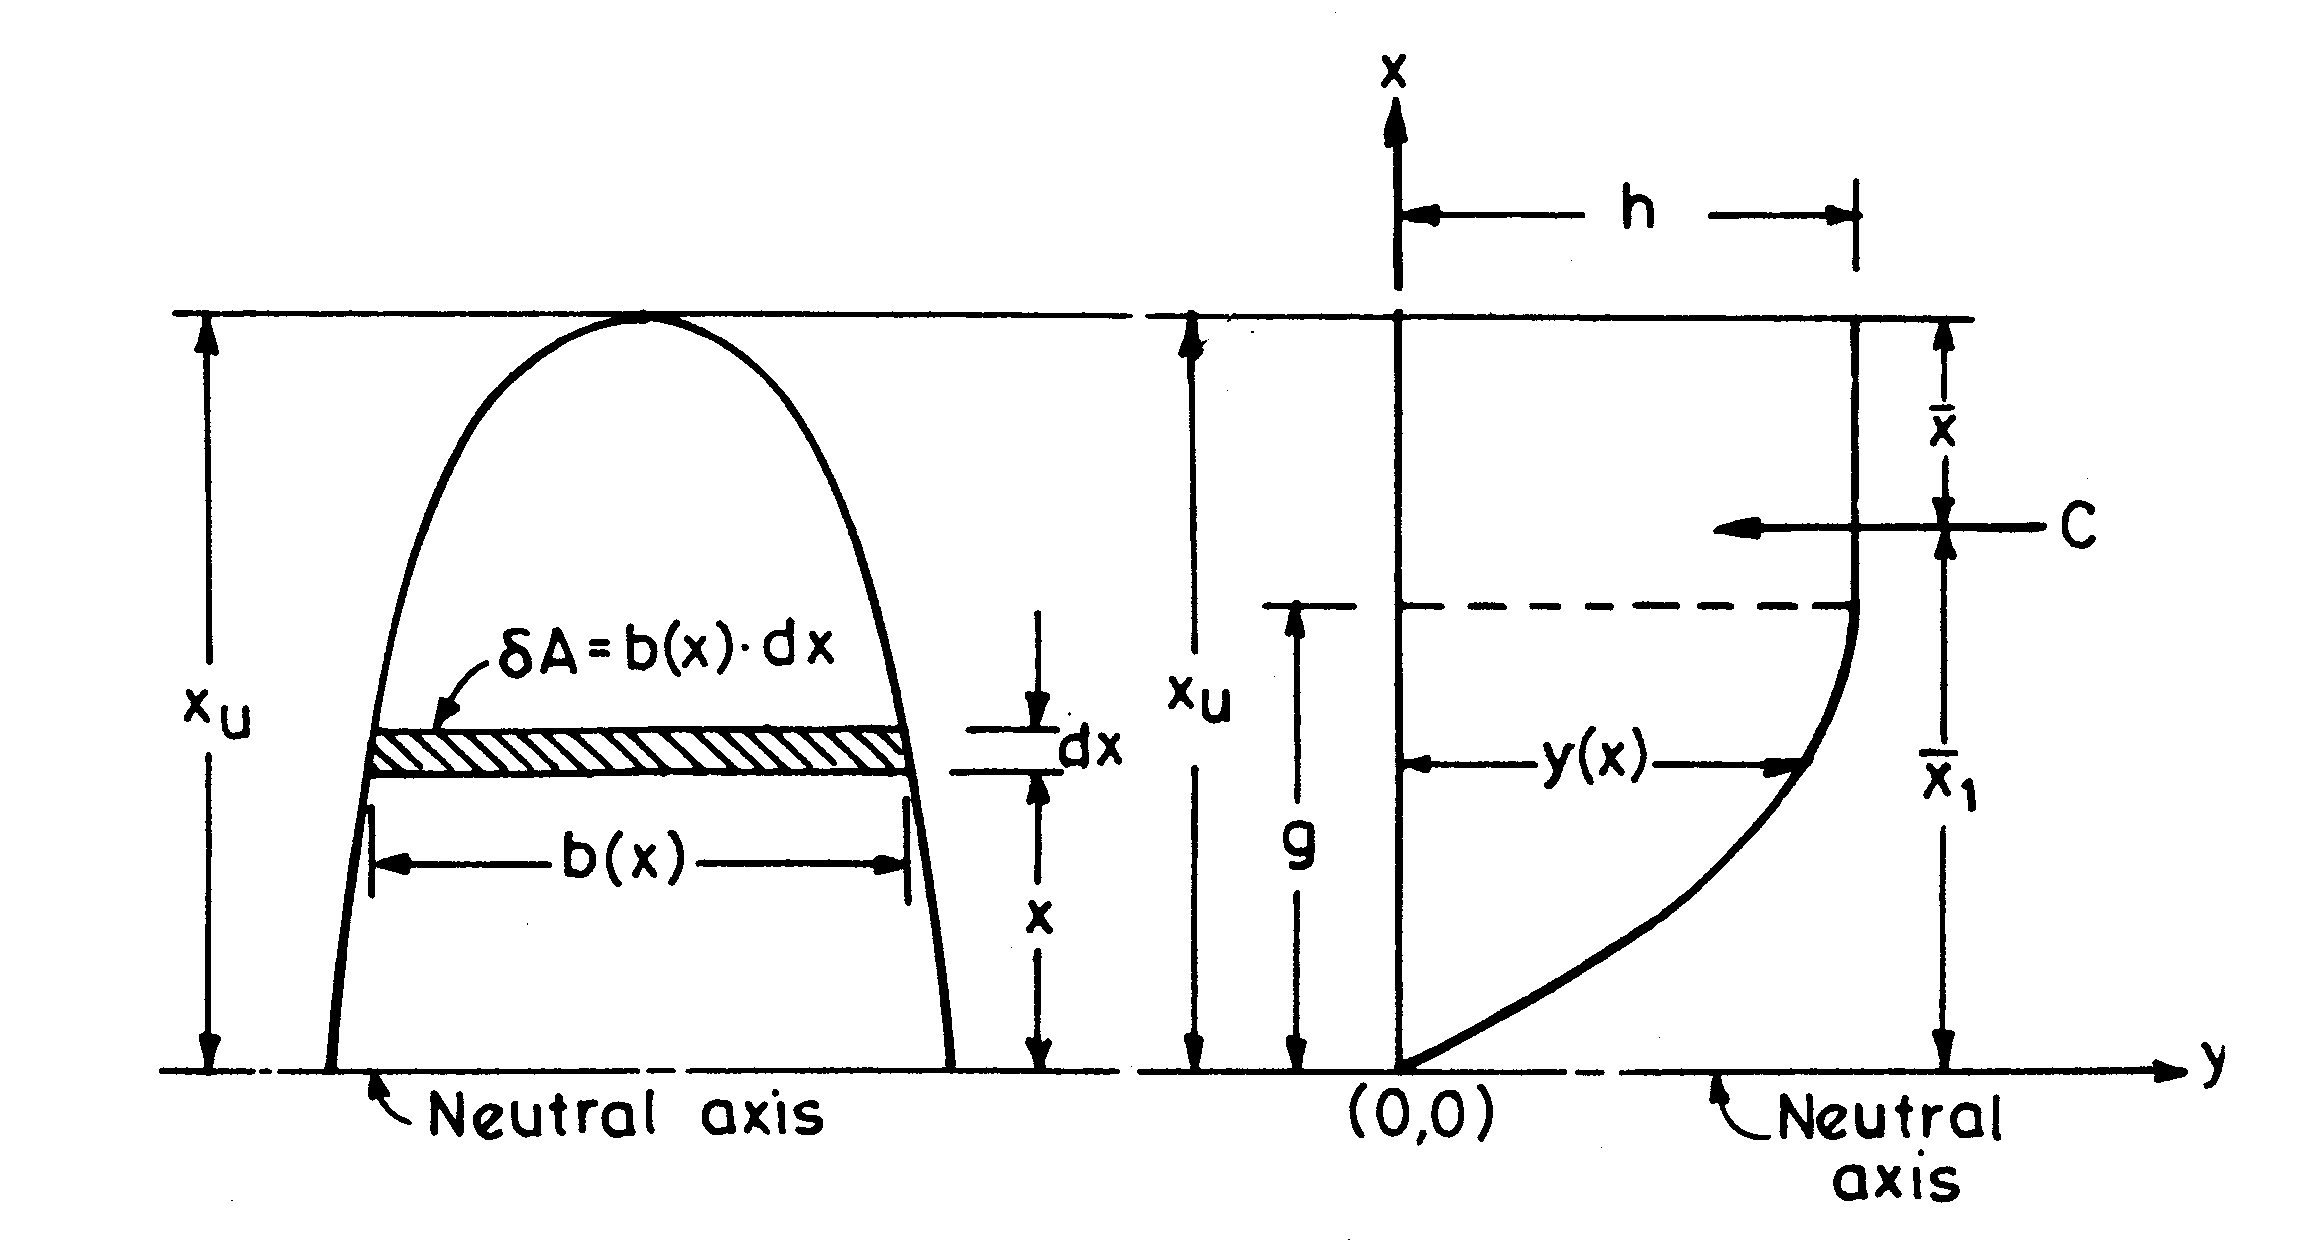
\includegraphics[width=0.5\textwidth]{images/concrete.png}
\caption{Concrete compression zone of any given shape under the stress diagram of the Code}
\label{fig:concrete}
\end{figure}

\begin{align}
C=\int_{x=g}^{x=0}b(x).y(x).\,dx+\int_{{x=x_u}}^{x=g}b(x).h.\,dx\\
C.(\bar x_1)=\int_{x=g}^{x=0}b(x).y(x).x.\,dx+\int_{{x=x_u}}^{x=g}b(x).h.x.\,dx
\end{align}

The location of the concrete compressive force from the top fiber of 
section is given by (\fig 1.2),
\begin{equation}
\bar x=x_u-\bar x_1
\end{equation}
\eqn ( 1.8) to \eqn (1.10) are applied to rectangular and triangular
shapes of concrete compression zone and the results are given in \fig 1.3.

When the concrete stress diagram is only a part-parabola (\fig 1.4), 
the expressions for the area (A) of the stress diagram and the location
of its centre of gravity ${(\bar x)}$ from the top fibre of section are
given below.

\begin{figure}
\centering
\begin{subfigure}{0.5\textwidth}
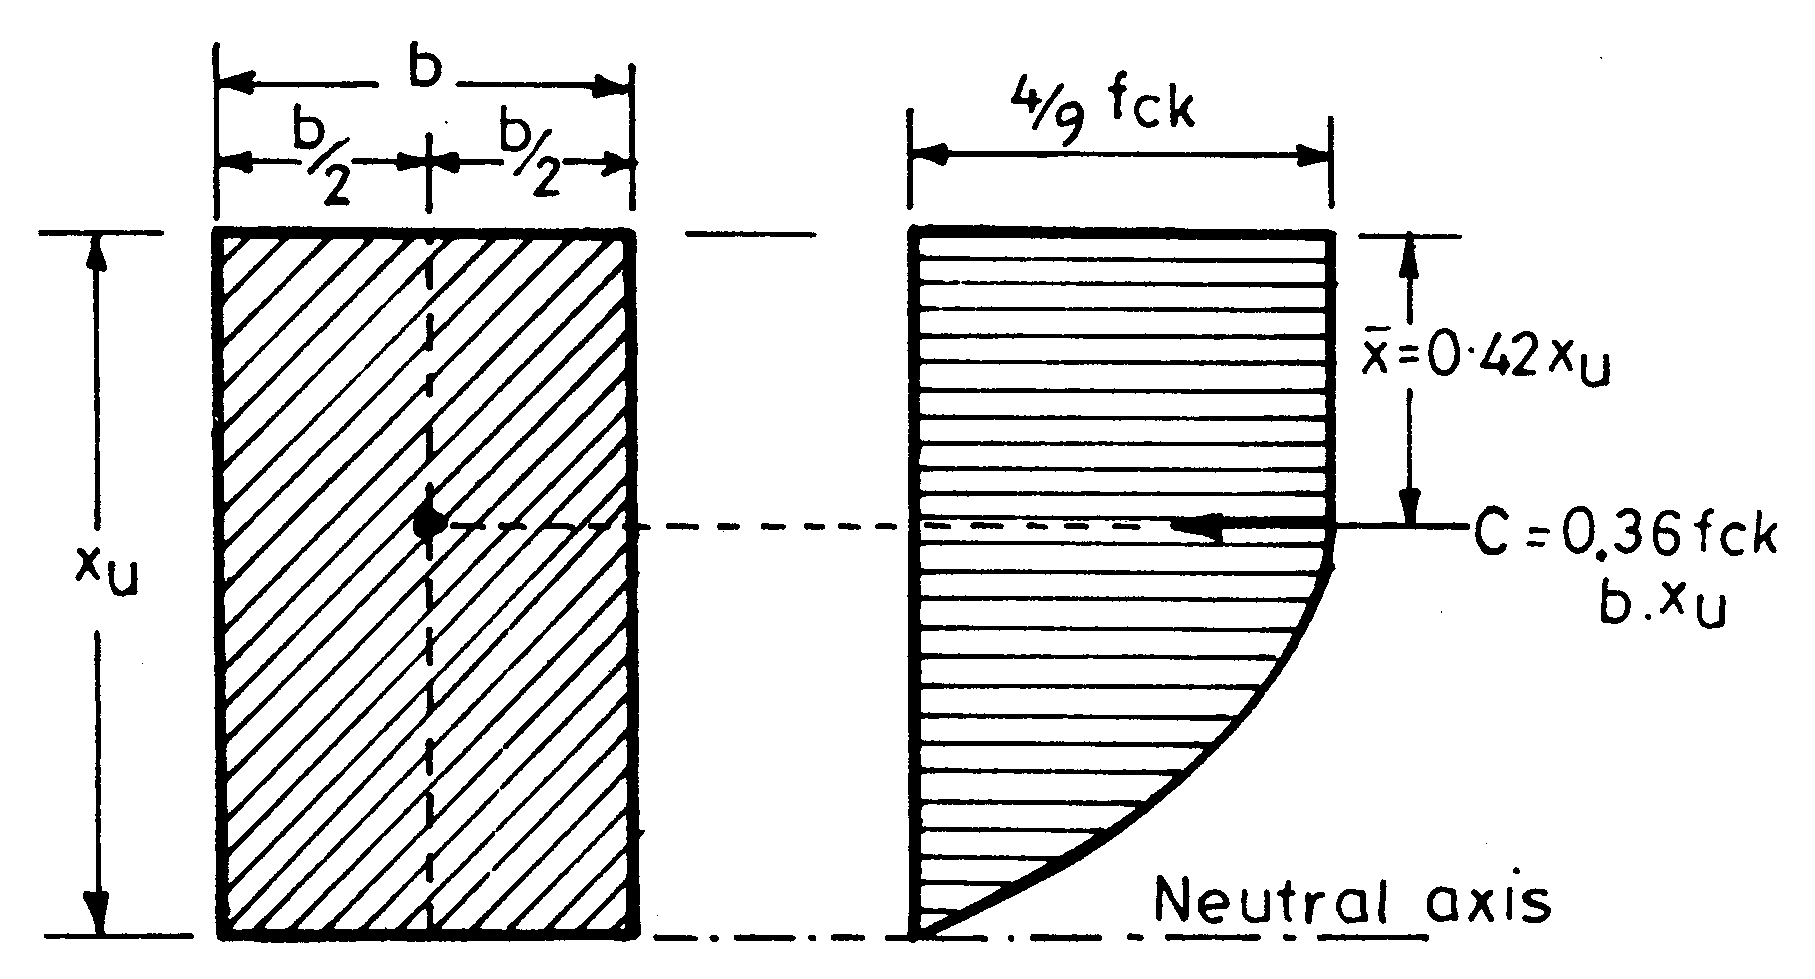
\includegraphics[width=\textwidth]{images/rectangular.png}
\caption{Rectangular concrete compression zone.}
\label{fig:rectangular}
\end{subfigure}
%
\begin{subfigure}{0.5\textwidth}
\centering
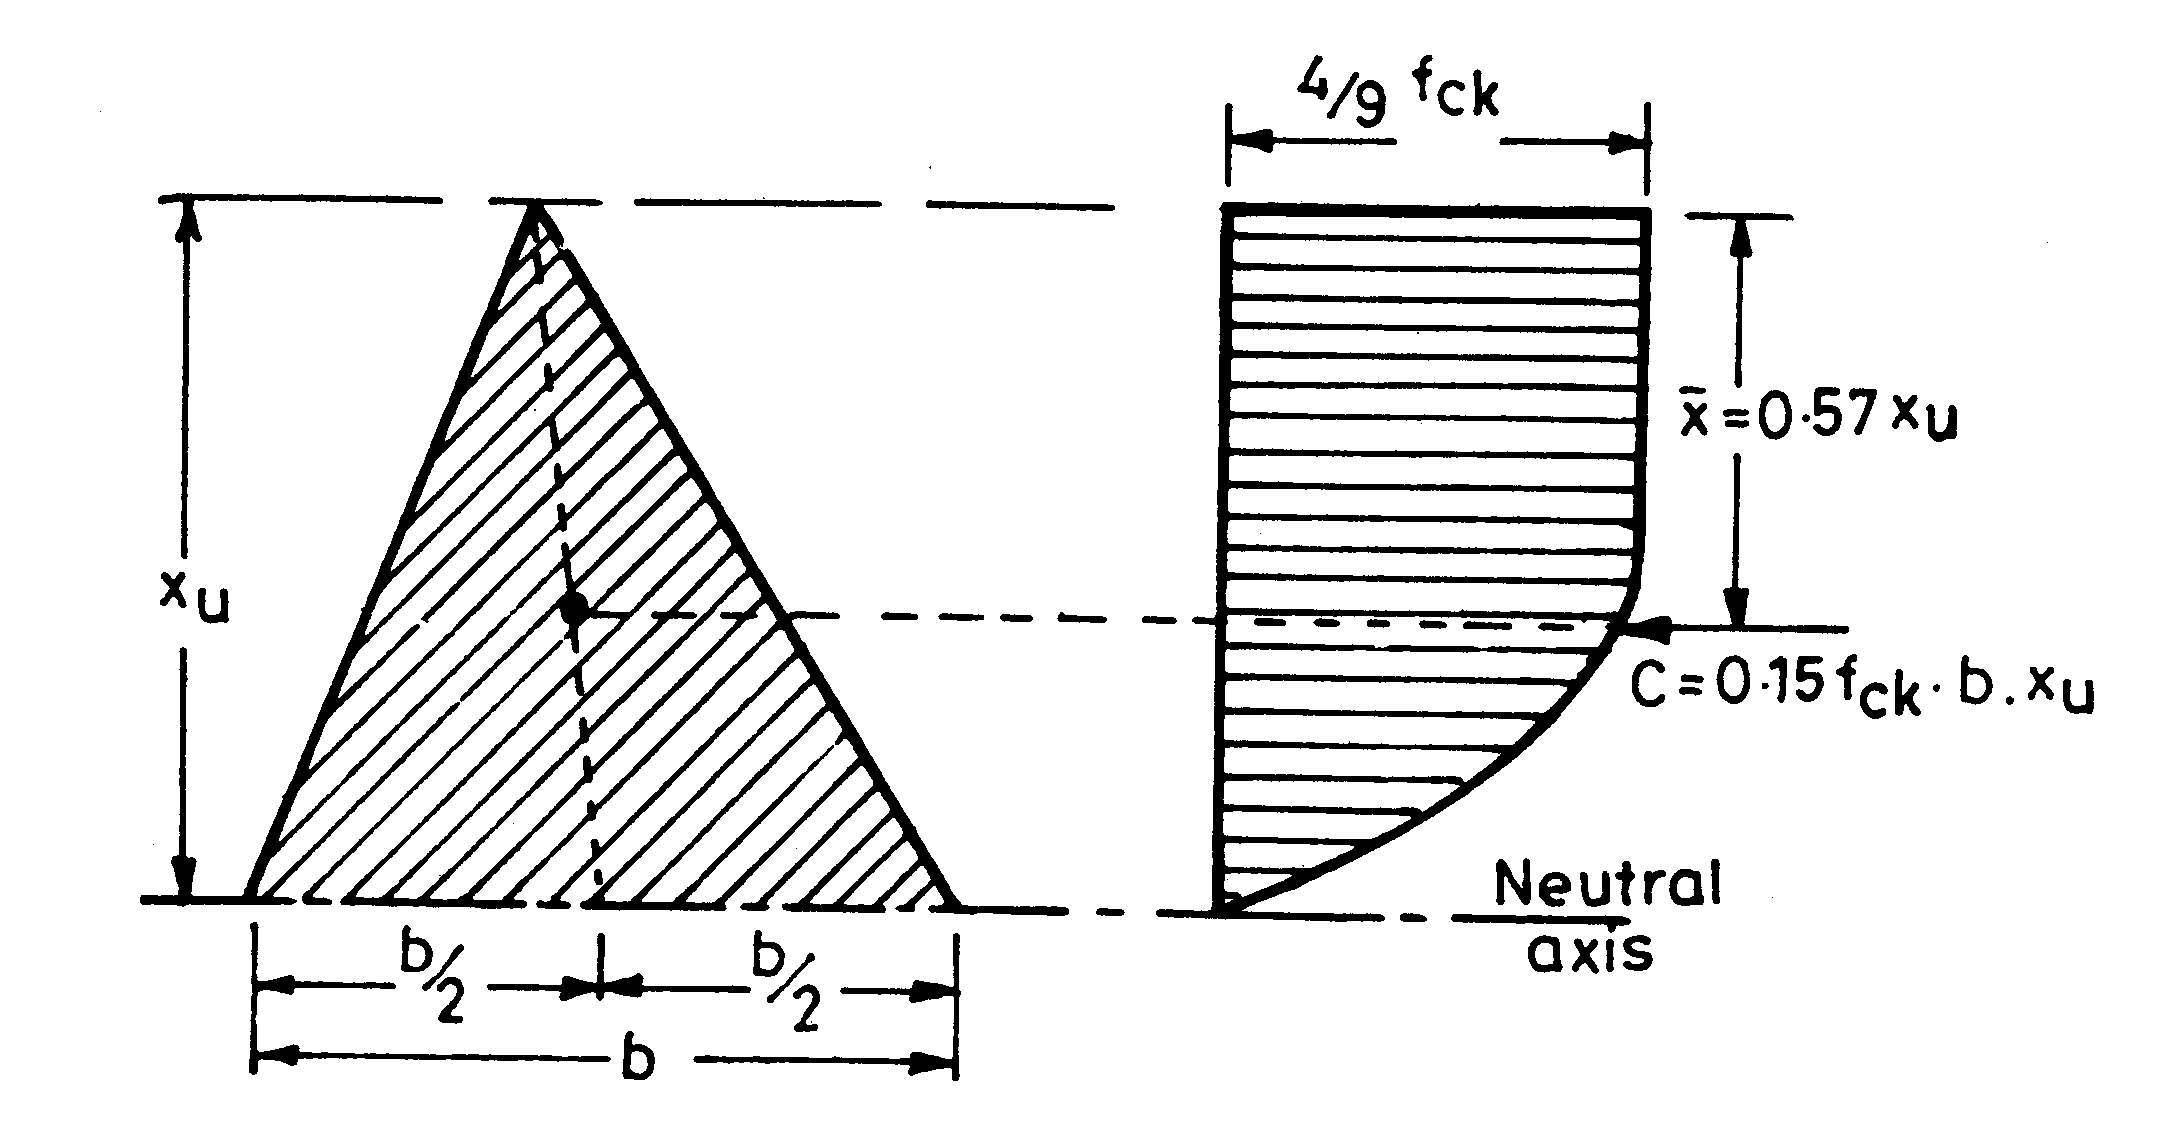
\includegraphics[width=\textwidth]{images/triangular.png}
\caption{Triangular concrete compression zone.}
\label{fig:triangular}
\end{subfigure}
%
\begin{subfigure}{0.5\textwidth}
\centering
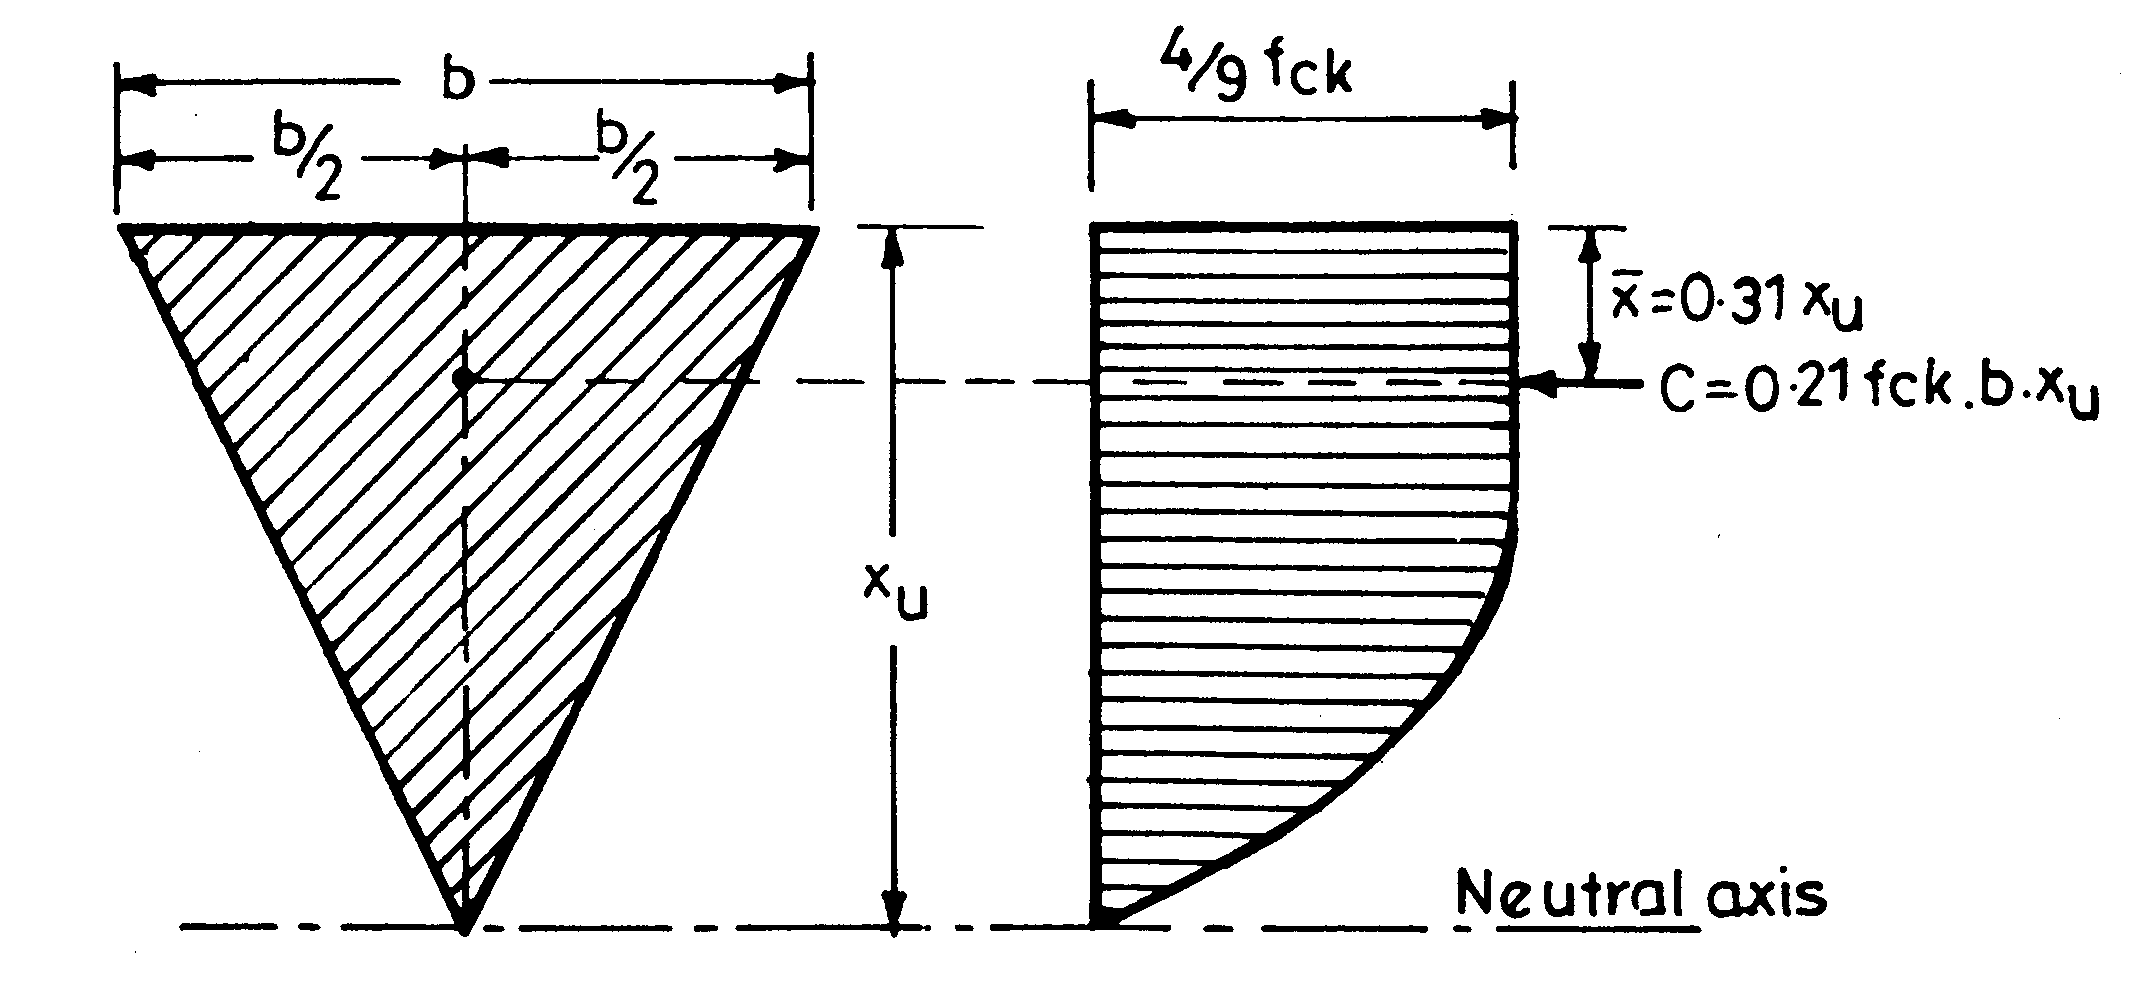
\includegraphics[width=\textwidth]{images/inverted.png}
\caption{Inverted triangular concrete comparison zone.}
\label{fig:inverted}
\end{subfigure}
\caption{Concrete stress block parameters for three basic shapes of concrete compression zone.}
\label{fig:concrete}
\end{figure}

\begin{align}
\frac{x_u}{g}=\frac{\epsilon}{0.002}\\
A=-\frac{1}{3}.\frac{h}{g}^2.x_u^2+\frac{h}{g}.x_u^2\\
A.\bar{x}=-\frac{1}{4}.\frac{h}{g}^2.x_u^4+\frac{2}{3}.\frac{h}{g}x_u^3\\
\bar{x}=-x_u-\bar{x_1}\\
f_c=-\frac{h}{g}^2.x_u^2+2.\frac{h}{g}.x_u
\end{align}

When the neutral axis falls below the section, the expressions for the
area (A) of the concrete stress diagram and the location of its centre
of gravity $(\bar x)$ are given below (\fig 1.5).
\iffalse

\begin{align}
j=0.45f_{ck}\left(\frac{4}{7k-3}\right)^2\\
A=0.45f_{ck}D-\frac{4}{21}.j.D\\
A.\bar{x}=0.45f_{ck}.\frac{D}^2{2}-\FRAC{8}{49}.j.D^2\\
\end{align}
\fi
\fig 23 of the \citetitle{is4562000} gives stress-strain curves for
steel types  (ordinary mild steel plain bars) and {\fefouronefive} and
{\fefivezerozero} (high strength steel deformed bars) with the modulus ofelasticity
of steel being $E_s = 2*10^5 N/mm^2$, which is given to be the same
for all types of reinforcing steel.The design strength of steel, equal
in both tension and compression,is given by,

\begin{figure}
\begin{subfigure}{0.3\textwidth}
\centering
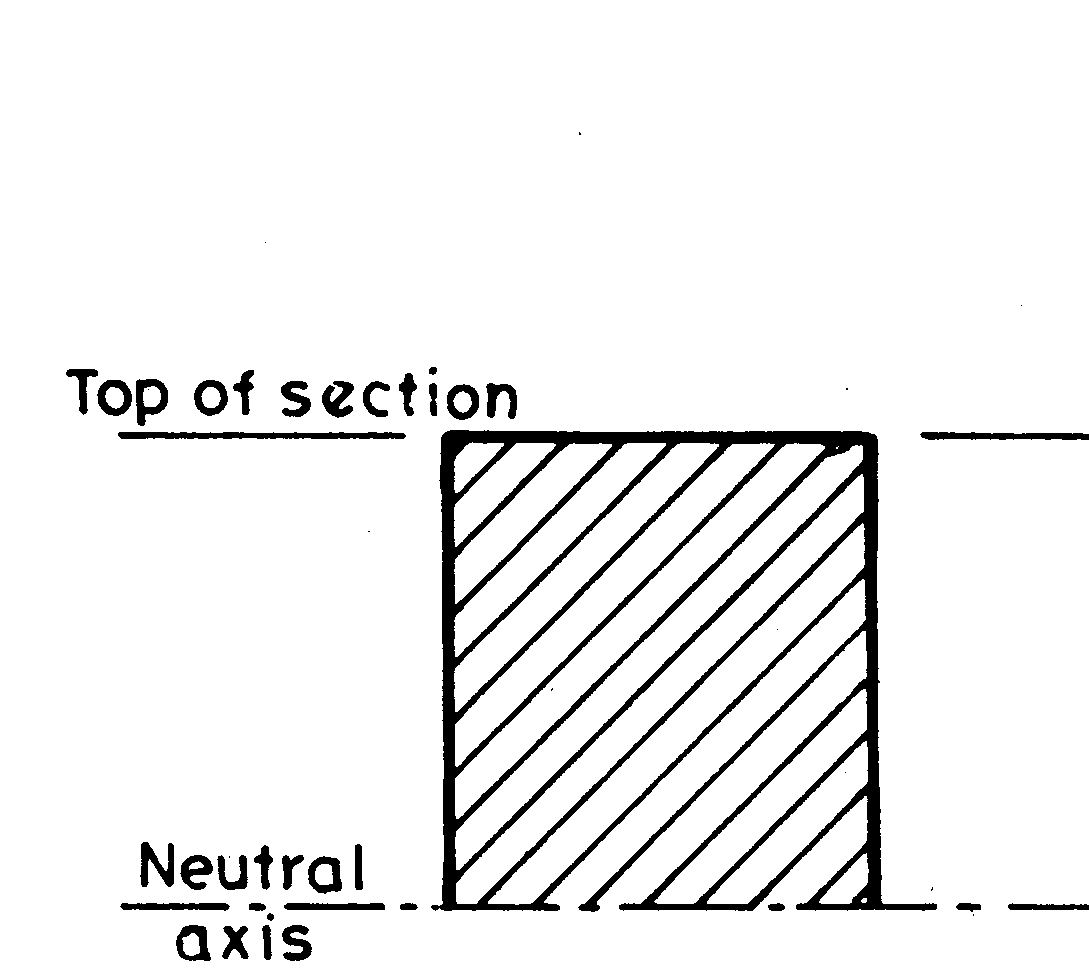
\includegraphics[width=\textwidth]{images/compressiona.png}
\caption{Concrete compression zone}
\label{fig:compression}
\end{subfigure}
%
\begin{subfigure}{0.3\textwidth}
\centering
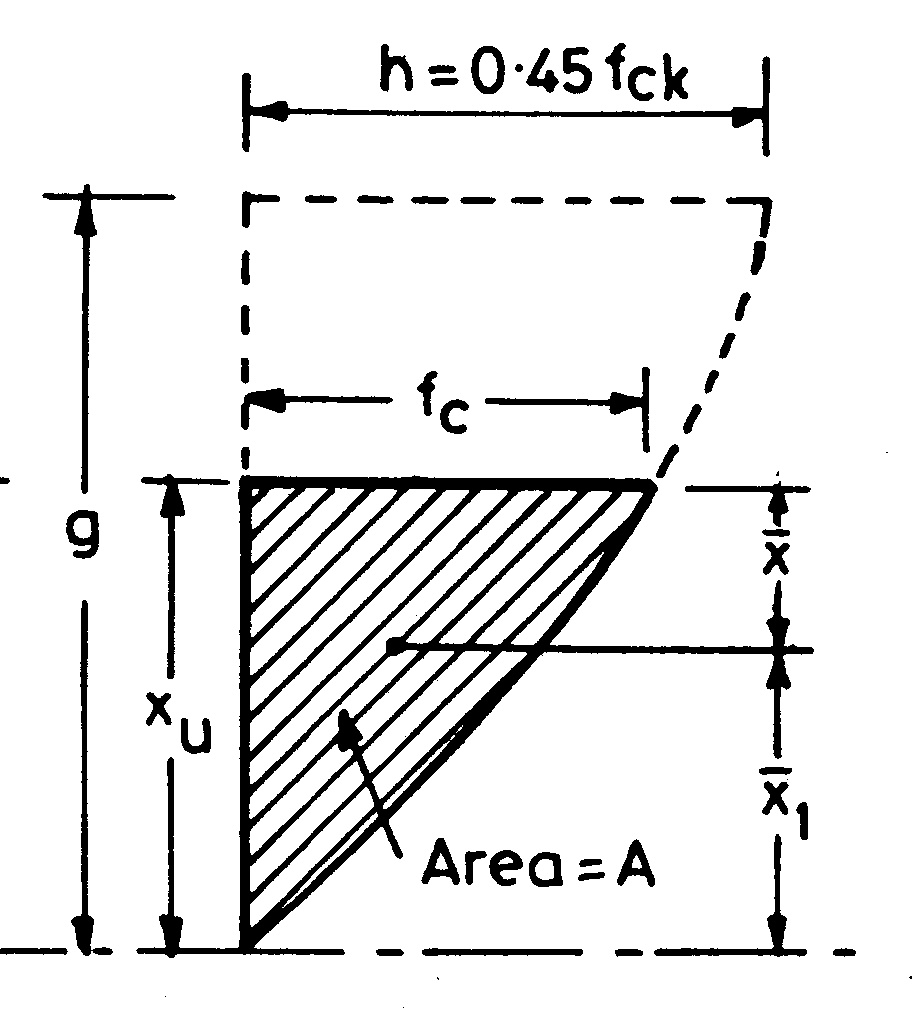
\includegraphics[width=\textwidth]{images/concretestressb.png}
\caption{Concrete stress diagram part-parabola}
\label{fig:stress}
\end{subfigure}
%
\begin{subfigure}{0.3\textwidth}
\centering
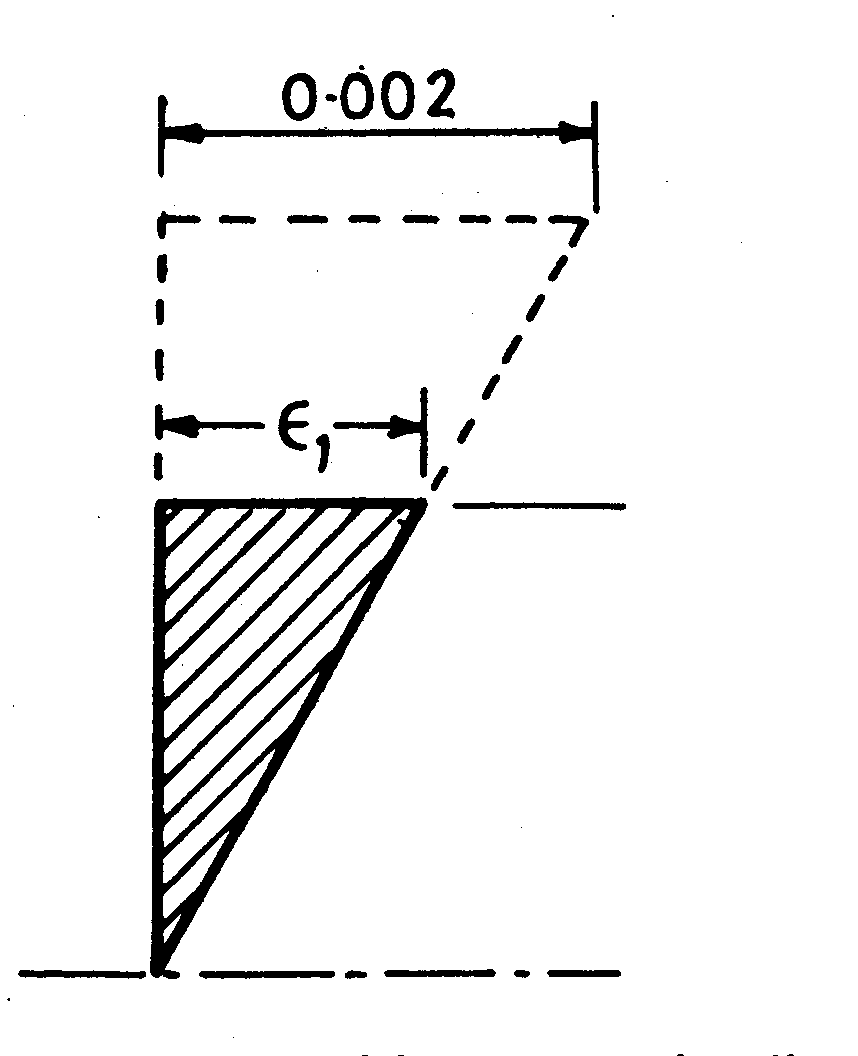
\includegraphics[width=\textwidth]{images/linearstrainc.png}
\caption{Linear strain diagram}
\label{fig:strain}
\end{subfigure}
\caption{Part-parabolic concrete stress diagram}
\label{fig:part}
\end{figure}

\begin{equation}
f_s=\frac{f_y}{\gamma_m}=\frac{f_y}{1.15}=0.87f_y
\end{equation}

where, fy is the characteristic yield strength of steel, as shown in
\fig 23 of the \citetitle{is4562000}. \tablem 1.1 gives values of design
stresses in steel type {\fefouronefive} for various strain values.
This table is used extensively for developing design aids for steel
type {\fefouronefive}. In this manual, no separate design aids are given
for steel type {\fefivezerozero}. As the stresss-strain diagram for
{\fefivezerozero} is similar to that for {\fefouronefive} and as the difference in
the yield stresses of the two steel types is small, it is seen that. 
steel area for {\fefivezerozero}  in the design of reinforced concrete 
sections can always be found with reasonable accuracy by using design
aids for steel.

\begin{figure}
\centering
\begin{subfigure}{0.3\textwidth}
\centering
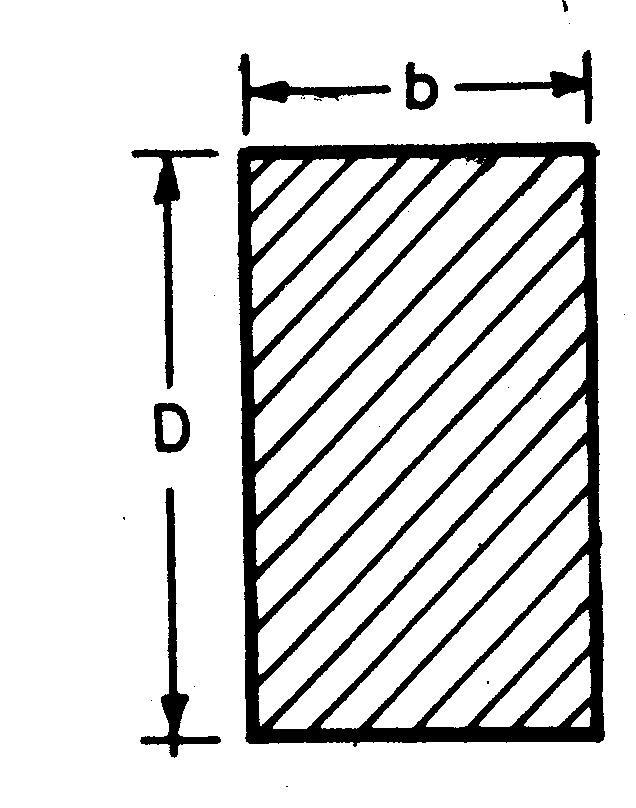
\includegraphics[width=\textwidth]{images/sectionfullya.png}
\caption{Section fully under compression}
\label{fig:section}
\end{subfigure}
%
\begin{subfigure}{0.3\textwidth}
\centering
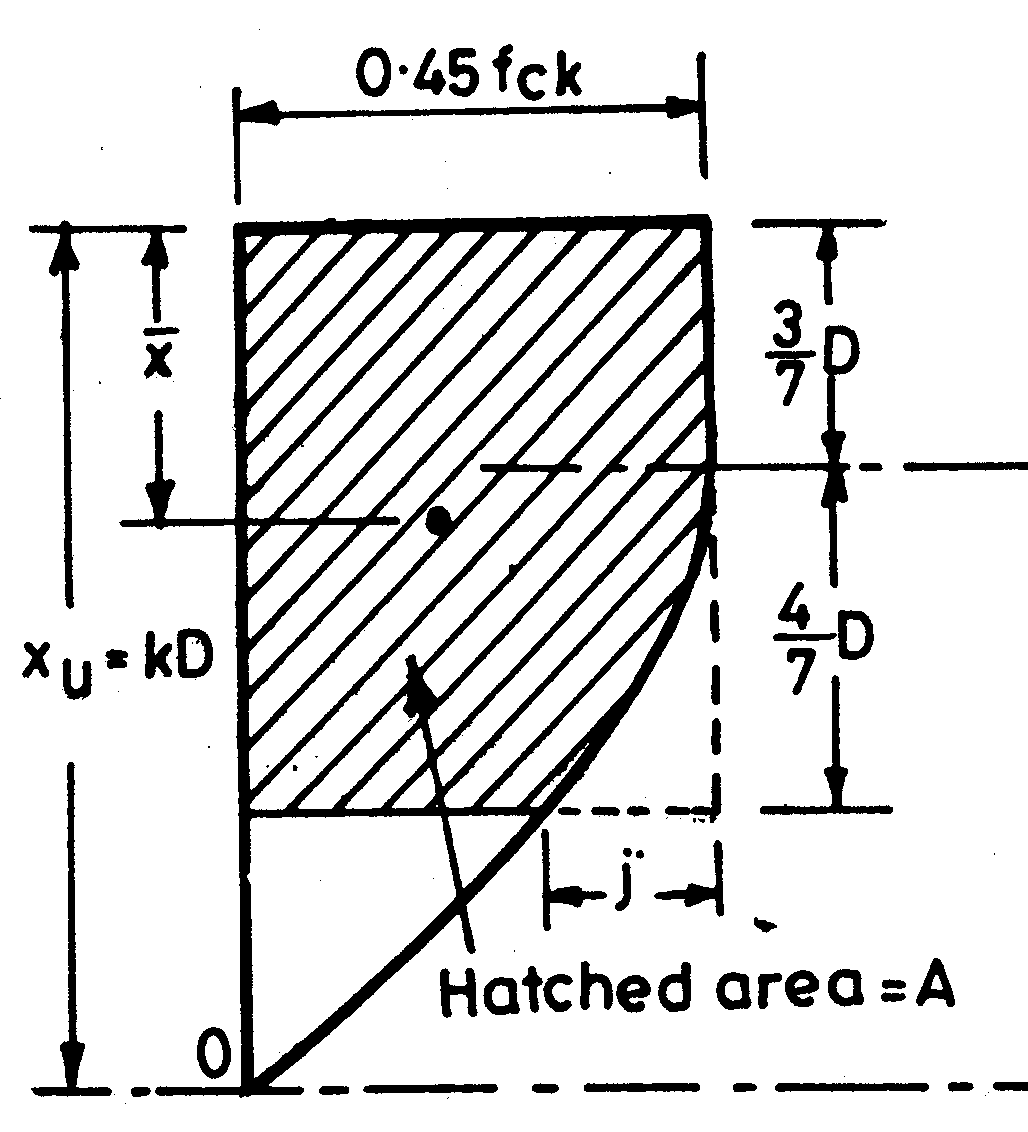
\includegraphics[width=\textwidth]{images/concreteb.png}
\caption{Concrete stress diagram}
\label{fig:sec}
\end{subfigure}
%
\begin{subfigure}{0.3\textwidth}
\centering
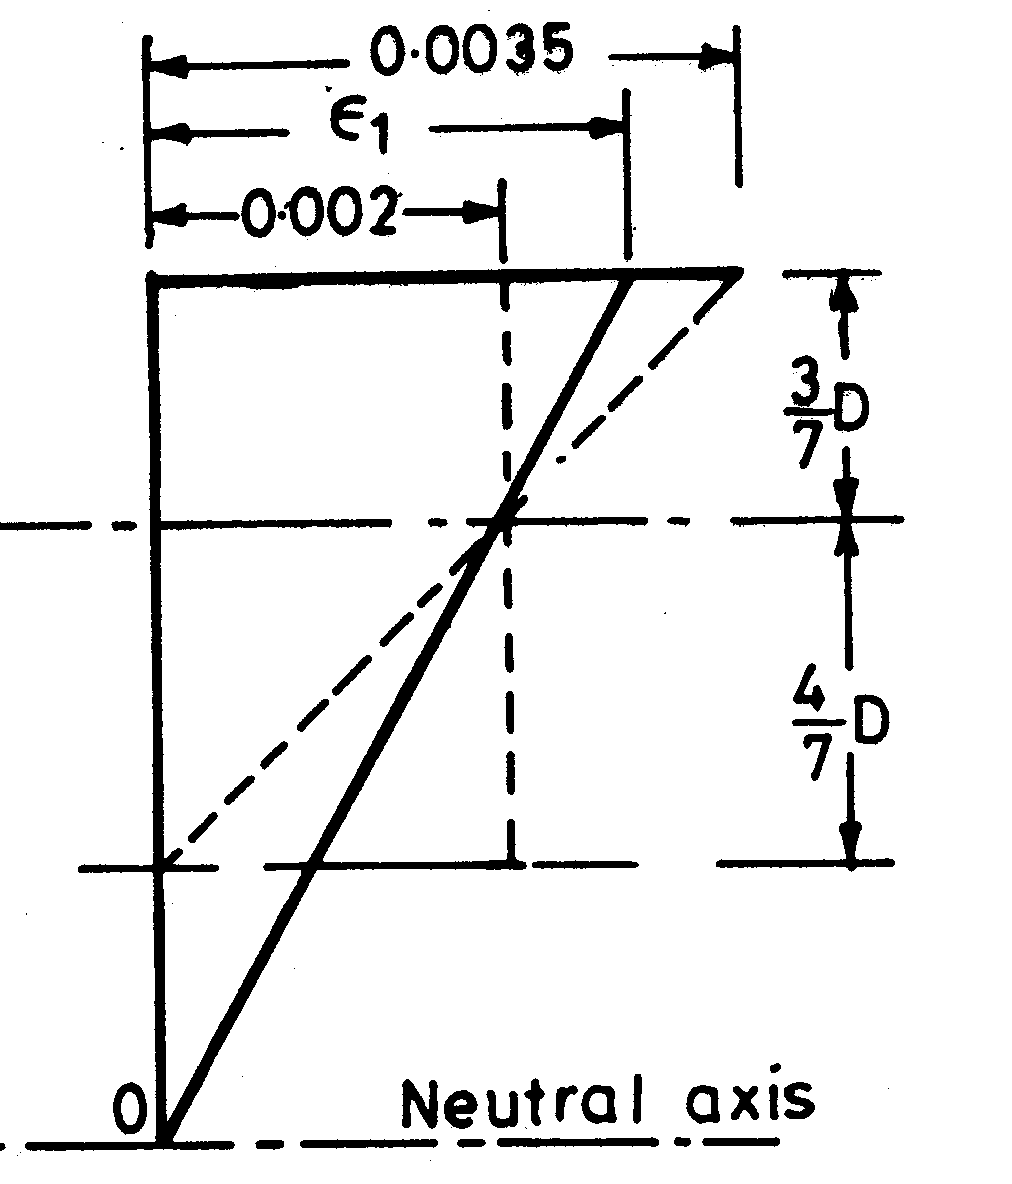
\includegraphics[width=\textwidth]{images/conretestraiinc.png}
\caption{Concrete strain diagram}
\label{fig:con}
\end{subfigure}
\caption{Concrete stress block parameters when netural Axis is below the section}
\label{fig:block}
\end{figure}

type {\fefouronefive} and using a $multiplier=\frac{415}{500} = 0.83$ to the steel
area obtained for {\fefouronefive}. Thus, for all reinforced concrete members,
design aids are givenonly for the two steel types {\fetwofivezero} and
{\fefouronefive}.

\section{Behaviour of Reinforced Concrete Members at Failure}

A member under bending with or without axial load of either comperssive
or tensile nature may fail under either of the following three modes of
failure 4.

\begin{enumerate}[(i)]
\item Tension failure.Concrete crushed or not crushed,but tension steel well in yield.
\item Balanced failure.Concrete crushed and tension steel just in yield.
\item Compression failure.Concrete crushed and tension steel not in yield.
\end{enumerate}

With a very low amount of tension steel, failure will be initiated by
yielding of reinforcement and collapse will take place with snapping of
reinforcement at the ultimate elongation , of steel (83m) as given by 
the breaking tests of different types of steel specified by relevant
codes5’ 6. “At this stage, strain in concrete at the extreme fibre of 
section (81) may be less than the maximum crushing strain of concrete
(0.0035). When the section is not excessively under-reinforced, failure
is initiated by the yielding of tension steel. Consequently, the neutral
axis shifts upwards and the final collapse is also associated with the
crushing of concrete. These two modes of failure fall under the category
of tension failure which takes place gradually and gives ample warning
before collapse.

When the amount of tension steel is large, the section is over-reinforced.
Then the concrete reaches its ultimate crushing strain $(\epsilon_{stu})$
before the tension steel starts yielding. This is called compression
failure and it leads to a sudden collapse without warning due to the
brittle nature of concrete. For this reason, it needs to be avoided or
provided for, in design based on limit state of collapse. Balanced
failure is just a transition between the tension and the compression
failures. In general, members should be so designed that tension failure
is ensured at the limit state of collapse. In order to achieve this, the
necessary criterion is that the tension steel must be well in yield. The
Code, in its clause 38.1 (f) has, therefore, stipulated that the minimum
strain in the tension steel shall exceed the linear elastic yield strain
by 0.002. This ensures that the tension steel of a type with fixed yield
point like {\fetwofivezero} will definitely be in yield, thereby, giving ductility
to the number. In cold worked steels like {\fefouronefive} and
{\fefivezerozero}, the yield stress is associated with steel strain equal to
$\epsilon_{std}=\frac{f_y}{1.15 E_s}+0.002$, thereby, satisfying the
above requirement of the Code. Members under axial compression with or
without moment fail under compression failure.This can not be avoided.
But in order to reduce the suddenness and explosion of this type of
failure, concrete crushing strain is reduced from 0.0035 to 0.002 and
lateral ties are provided in members to improve ductility.

\section{Unified Approach}

It would be ideal to consider a member under bending and axial load
$(P_u, M_u)$ as a general case, of which a beam $(P_u=0,M_u)$, a column
$(+ve P_u,M_u)$ and a tension member $(—ve P_u,M_u)$ form only particular
cases. This may be called a unified approach.The Code,in its Section 5 on
the limit state method of structural design, has giVen a limited unified
approach for members under bending combined with axial compression but
has made no mention of tension members. SP-16 $Design Aids^8$ have
however,given charts for design of tension members with equal steel on
opposite faces or equal steel on all four faces, without making clear the
basis of their development.The old code had given separate treatments for
beams,columns and ties giving no unified approach for their design. There
is no doubt that these different members behave under load in special
patterns but it is quite fascinating to include all these special
patterns into a unified approach so that design aids can be developed
which can be used with equal ease for design of beams, columns as well 
as tension members. The compartmentalised approach for beams, columns
and ties has led to proliferation of design aids and loss of continuity,
clarity and conciseness in design. Further, the unified approach can be
extremely useful for design of reinforced concrete sections subject to
biaxial bending combined with axial load of either nature.

For the limit state of collapse for bending and axial compression, the
Code lists the relevant assumptions in clauses 38.1 and 39.1. For the
limit state of collapse for bending combined with axial tension, the
following additional assumptions are made.

\begin{enumerate}[(i)]
\item The minimum tensile strain in axial tension is taken equal to $\epsilon_{std}$,
\begin{equation}
where, 
\epsilon_{std}=\frac{f_y}{1.15{\epsilon_s}}+0.002
\end{equation}
\item  For bending combined with axial tension, the maximum tensile
strain in the most highly stretched steel layer shall be equal to 1/10th
the ultimate elongation $(\epsilon_{stu})$ which is given by the tensile
tests of different types of steelas stipulated in relevant
$codes^{5,6}$.This gives,
\end{enumerate}
\begin{equation}
\epsilon_{st},max=\frac{1}{10}.\epsilon_{stu}
\end{equation}

The maximum tensile strain in steel is not given by the Code. The obvious
value for the maximum tension steel strain is its snapping strain 83m. But
the values of snapping strains for steel types Fe 250,Fe 415 and Fe 500 are
quite high.Therefore,in order toput a limit on excessive cracking and
spalling of concrete of tension zone, it is assumed that the maximum
tensile strain may be limited to 1/10th the snapping strain of steel.For 
steel types {\fetwofivezero}, {\fefouronefive} and {\fefivezerozero}, this 
assumption gives values of 0.020, 0.0145 and 0.012 respectively for
the maximum tensile strains.
These values compare well with 0.005 and 0.01 assumedfor all types of
reinforcing steel by DIN $1045^9$ and CEB Model $Code^{10}$ respectively.
Further, the requirement for ensuring ductility in sections,
$$\epsilon_{st}=\epsilon_{std}=\frac{f_y}{1.15 E_s}+0.002$$
has been given by the Code for tension failure of beams only. In the
unified approach, this requirement of ductility is extended to tension
failure of sections under bending with or without axial load of either
compressive 0r tensile nature. As it is known that a ductile tension
failure is a gradual one and gives ample warning before collapse, it
is advantageous to ensure ductility for all members (not only for beams) 
under tension failure.

With these additional assumptions, a section under bending combined with
axial load of either compressive or tensile nature can be analysed for
its full range of variation of axial load from
$+P_u(compression) to -P_u (tension)$ with pure bending case $(P_u=0)$
following as a transition. The design assumptions for a section under
bending and axial load are portrayed in Fig. 1.6, by the various strain
diagrams applicable for the full range of variation of Pu.

\begin{figure}
\centering
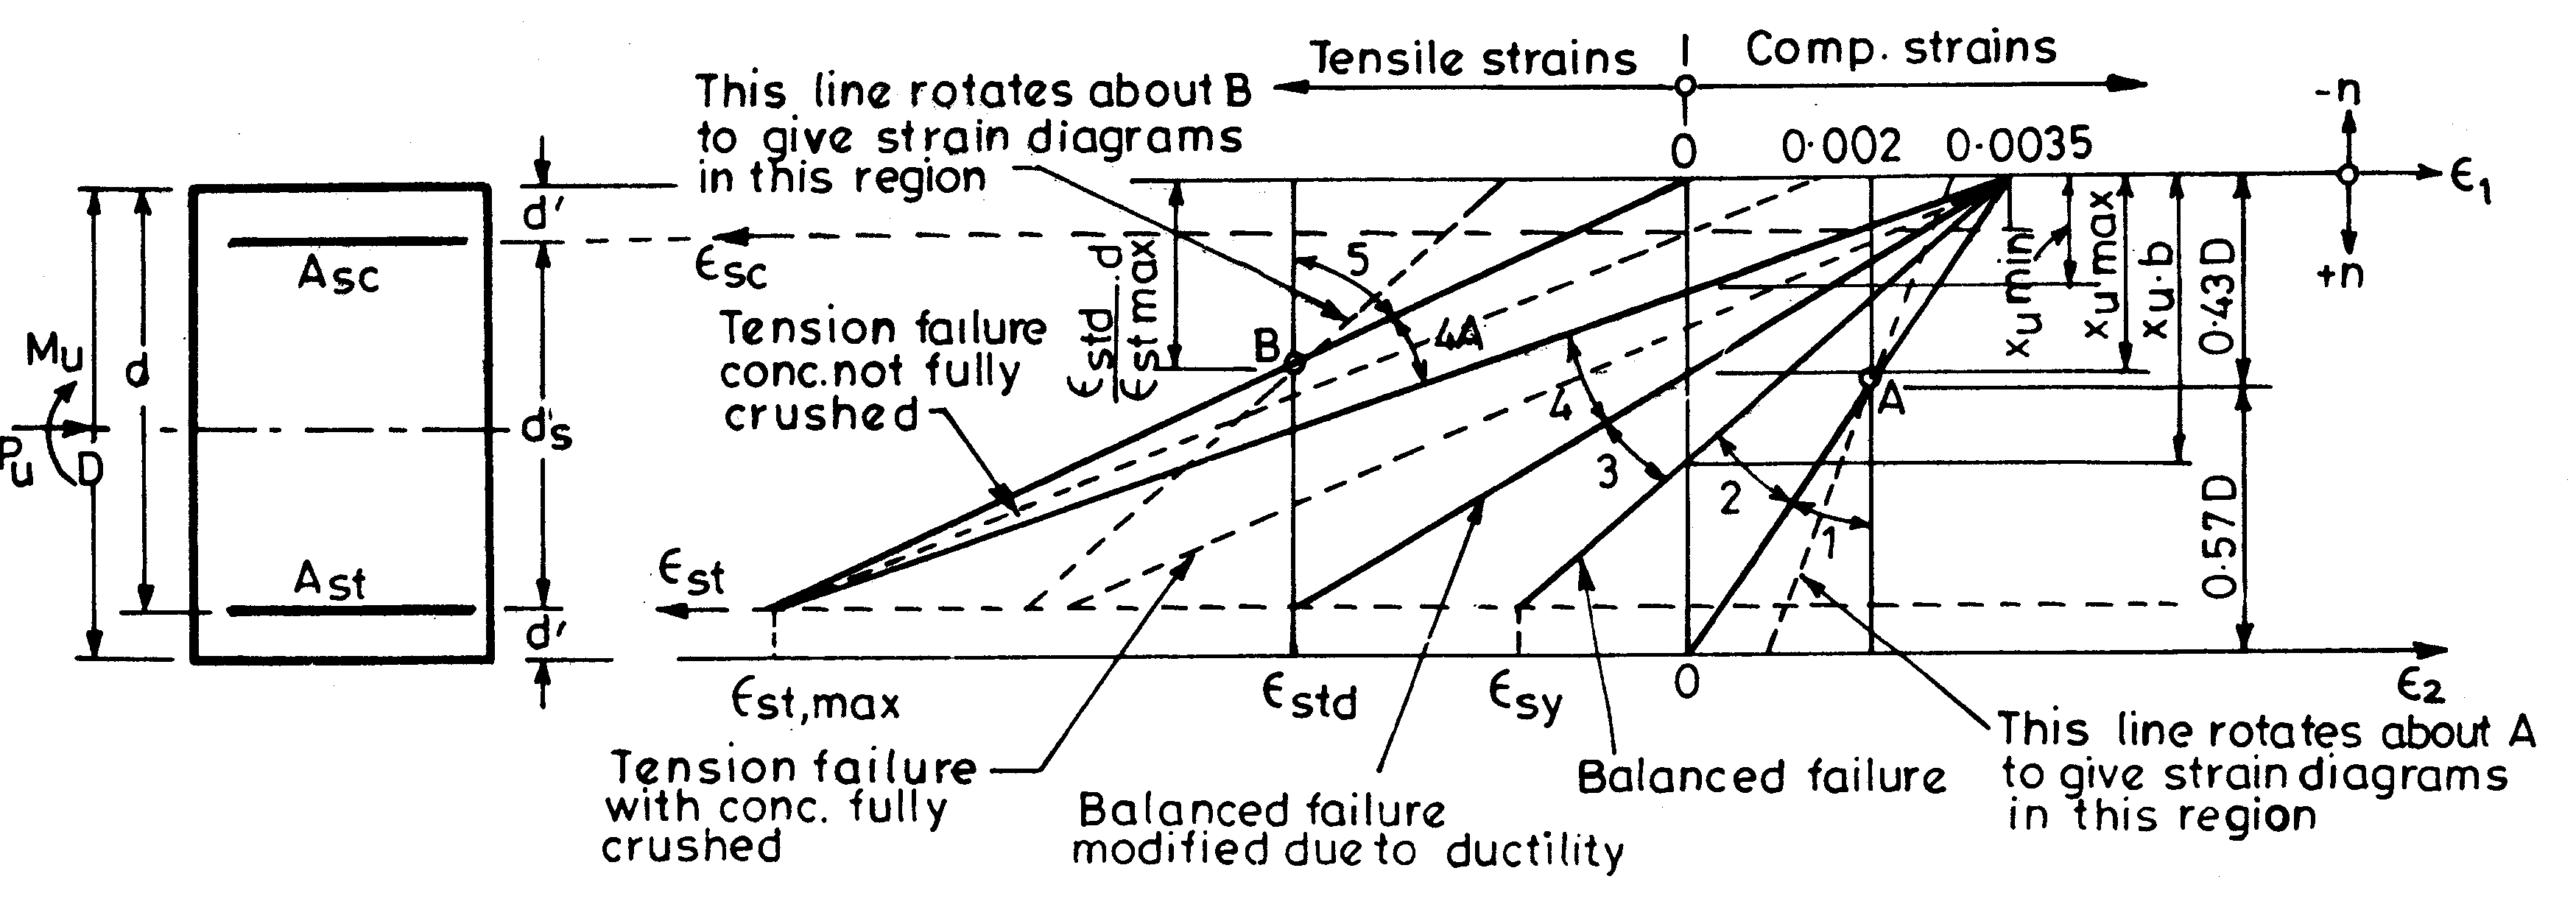
\includegraphics[width=0.6\textwidth]{images/various.png}
\caption{Various strain diagrams applicable for a section under bending and axial load.}
\label{fig:various}
\end{figure}

For a section under bending combined with axial compression, clause 39.1 (b) of the Code
gives the equation,
\begin{equation}
\epsilon_1=0.0035-0.75\epsilon_2
\end{equation}
which represents various strain diagrams given in the line rotating about
the point A (\fig 1.6). On a similar analbgy, the line rotating about the
point B (\fig 1.6) gives different strain diagrams applicable for a
section under bending combined with axial tension, which can be got from
the following relations for different types of reinforcing steel.

\begin{align}
For 
Fe 250,\epsilon_{st}=0.0020-5.45\epsilon_1\\
Fe 415,\epsilon_{st}=0.0145-2.82\epsilon_1\\
Fe 500,\epsilon_{st}=0.012-1.86\epsilon_1
\end{align}

The above relationships have been derived by using the principles of
similar triangles along with the values of $\epsilon_{st}, max, \epsilon_{std}$
for various types of steel given in \tablem 1.2. Figure 1.6 gives by
similar triangles,

\begin{equation}
n=\frac{\epsilon_1}{\epsilon_1+\epsilon_{st}}
\end{equation}

$n_b (balanced), n_max, n_min$ are calculated by the \eqn 1.26 and are
given in \tablem 1.2 for ready reference. Balanced failure is given by
$\epsilon_1 = 0.0035, \epsilon_{st} =\epsilon_{sy}$ ($\epsilon_{sy}$
corresponds to a steel strain when $f_{st} = 0.87 f_y$, to be read from
stress-strain curves for steel given in \fig 23 of the
\citetitle{is4562000}, balanced failure modified for ductility is given for
$\epsilon_1 = 0.0035, \epsilon_{st} = \epsilon-{std}$ and tension failure
with concrete not fully crushed is given for
$\epsilon_1 < 0.0035, \epsilon_{st} > \epsilon_{std}$. Tension failure 
with concrete not fully crushed is given for
$n < n_min, When \epsilon_{st} = \epsilon_{st}max and\epsilon_1 < 0.0035. When n .<= 0$, 
section is fully under tension and concrete strength is to be entirely
neglected and only steel areas are to be utilised to resist external
forces. When $n>n_b$, compression failure is indicated where concrete
is crushed $(\epsilon_1= 0.002 to 0.0035)$, but tension steel is not
yield, it may rather be in compression as well. \fig 1.7 shows typical
interaction curves for a section under bending and axial load with
different Regions 1 to 5 marked therein, which are also shown in fig 1.6.
The region-wise load moment combinations with corresponding strain values
are summarised below.

\begin{figure}
\centering
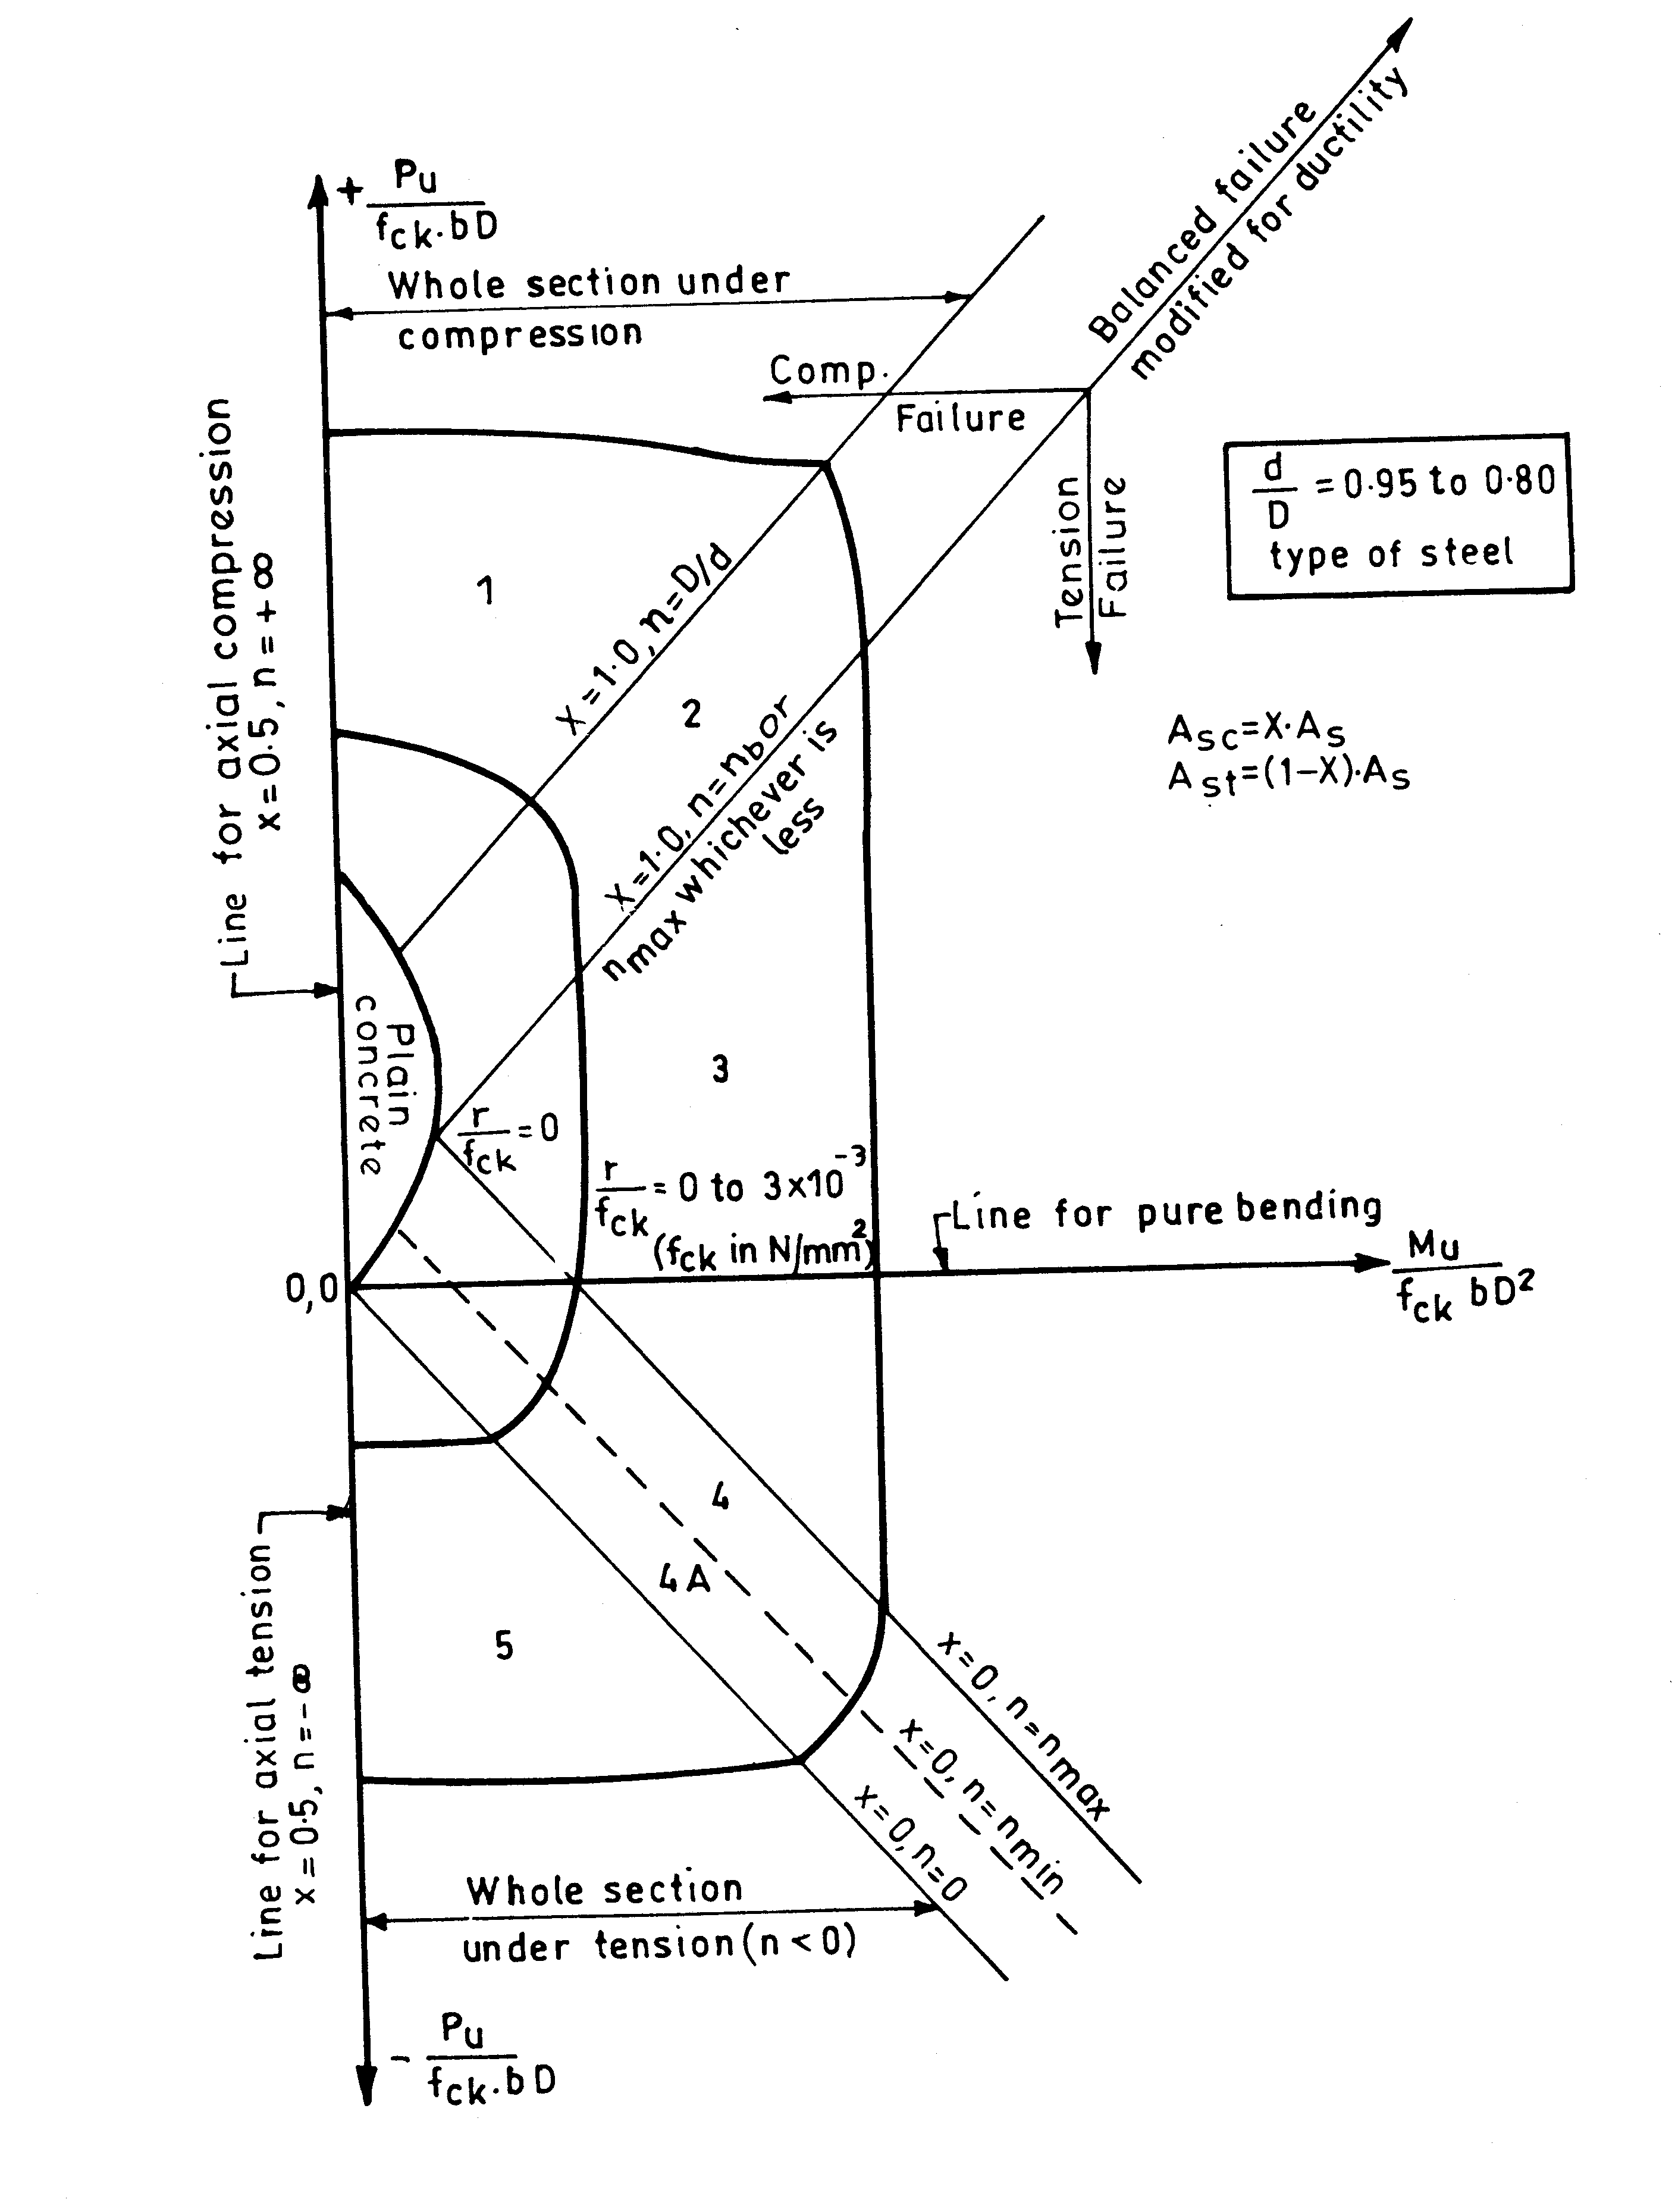
\includegraphics[width=0.5\textwidth]{images/exported.png}
\caption{Interaction curves for a section under bending and axial load.}
\label{fig:exported}
\end{figure}

Region 1. Whole section under compression, design governed by compression
failure with $\epsilon_1=0.002 to 0.0035, \epsilon_2=0 to 0.002 and n=\infty to D/d.$
pplicable for axial compression with or without small moment.\\

Region 2. Section partly under compression and partly under tension,
design governed by compression failure with
$\epsilon_1 = 0.0035 (constant) and \epsilon_{st} < \epsilon_{sy} and n = D/d to n_b.$
Applicable for axial compression with large moment.\\

Region 3. Section partly under compression and partly under tension,
design governed , by tension failure modified for ductility with

$$\epsilon_1 = 0.0035 (constant)$$
$$\epsilon_{st} =\epsilon_{sy} to \epsilon_{std} (theoretical)$$
$$=\epsilon_{std} (assumed constant for ductility).$$
$$n<= n_b$$
$$>n_{max} (theoretical)$$
But $$n=n_{max} (assumed constant for ductility).$$

This is a region when the value of X is not fixed.For a fixed arrangement
of steelin section,this region reduces to a straight line. \\

Region 4. Section partly under compression and partly under tension,design
governed by tension failure with concrete fully crushed with,

$$\epsilon_1 = 0.0035 (constant)$$
$$\epsilon_{st} = \epsilon_{std} to \epsilon_{st}, max$$
$$and n = n_{max} t0 n_{min}$$

Applicable for moment and axial load of either nature.
Region (4A) Section partly under compression and partly under tension,
design governed by tension failure with concrete not fully crushed with

$\epsilon_1 = 0 to0.0035, \epsilon_{st},\epsilon_{st},max(constant) and n = 0 to n_{min}$

Applicable for moment and axial load mostly tensile in nature.\\
Region 5. Whole section under tension, design governed by tension failure with 
$\epsilon_1 = 0 to \epsilon_{std} (tensile strains), \epsilon_{st}=\epsilon_{std}to \epsilon_{st}, max and n = 0 to — \infty.$
Applicable for axial tension with or without small moment.

\section{Analysis and Design of Structures}

In practice, structures are analysed by the well-known principles and
methods ofTheory of Structures under vertical and horizontal loads at the
working load level.There are distinct advantages in using working loads
during analysis of structures. Firstly, these give a realistic assessment
of loads on members and secondly, column loads are then directly usable
for design of footings, with the soil bearing capacity known at the working
load level.The choice of a common load factor of 1.5 for both dead and
live loads makes it easy to get ultimate forces which are used for
design of all critical sections in structural members. design of structural
members—slabs, beams, columns and footings—based on the limit state method 
in accordance with \citetitle{is4562000}. For each type of structural member, only
one type of design aid is given, which is chosen on the basis of its
effectiveness and convenience in practice. All design aids have been 
based on the governing formulae which have been fully derived and given
in the subsequentchapters. For a complete understanding of the subject,
this step. is quite important. Further, design aids are based strictly
on the theoretical development and do not incorporate in themselves other
design restrictions of the Code like minimum steel area in members, minimum
eccentricity and slenderness effects on columns etc. These effects are
dealt with separately outside the design aids. Design aids are developed
in such a way that these are effective for both design and review of
reinforced concrete sections. A unified approach for design of sections
under bending (both uniaxial and biaxial) and axial load of either
compressive or tensile nature is followed by which the same charts are
capable of being used for beams, columns and ties. Design aids are
prepared for two steel types {\fetwofivezero}  and {\fefouronefive} only.
Most design aids are made independent of concrete quality.

Numerical examples have been given to illustrate the use of design aids.
A consistent use of units for various quantities is important in analysis
and design of structures. With SI units, it is convenient to work out
loads in $kN/m^2$, moments and torques in or kNm, shears and column
loads in kN and soil pressures in $N/mm^2$ or $kN/cm^2$. The Code
gives values of all stresses $f_{ck}, f_y$ etc., in $N/mm^2$.'For working
out non-dimensional parameters like $\frac{P_u}{f_{ck}bD},\frac{M_u}{f_{ck}bD^2}$
etc.


It is a general practice to provide one type of reinforcing steel in a
building. This makes it easy for procurement of steel and supervision 
at the site. However, clause 26.1 of the Code permits use of two types
of reinforcing steel in a building, one for main reinforcement (say,
{\fefouronefive} or {\fefivezerozero}) and the other for stirrups in members
(say {\fetwofivezero}).
As the percentage increase in strength of the two types steel
\fefouronefive
(or {\fefivezerozero}) and {\fetwofivezero} is much greater than the percentage increase in
their costs, it is economical to use deformed steel bars
{\fefouronefive} (or \fefivezerozero) for both main and secondary
reinforcement in all members of buildings with the following two exceptions.

\begin{enumerate}[(i)]


\item Reinforcement in Slabs

Mild steel plain bars (Fe 250) should be used in slabs in order to reduce
slab thickness for control of deflection. For a general economy of the
building as a whole, thin slabs are preferable (Chapter 6). In practice,
Fe 415 steel is used in slabs with more steel provided at the midspan
in order to get less slab thickness.

\item Transverse Reinforcement in Columns

The pitch and diameter of lateral ties in columns are given in clause
26.5.3.2 (c) of the Code and these both are independent of steel quality.
{\fetwofivezero}, {\fetwofivezero} can, therefore, be used for lateral
ties in column for reasons of economy. Diameter 6 mm bars are rolled in
{\fetwofivezero} steel and these are used for column ties and stirrups in lintels.

Provision of more than one type of reinforcing steel in structural
members of a buildings calls for a careful planning and supervision at
the site.
\end{enumerate}
\section{Conclusion}

The general principles and the basic assumptions of the limit state
method of design of reinforced concrete structures are given in this
chapter, which are to be read in conjunction with the relevant clauses
of the Code.
